%!TEX root = ./template-skripsi.tex
%-------------------------------------------------------------------------------
%                            BAB III
%               			PEMBAHASAN
%-------------------------------------------------------------------------------

\chapter{METODOLOGI PENELITIAN}

\section{Keterhubungan Penelitian}

\begin{figure}[H]
	\centering
	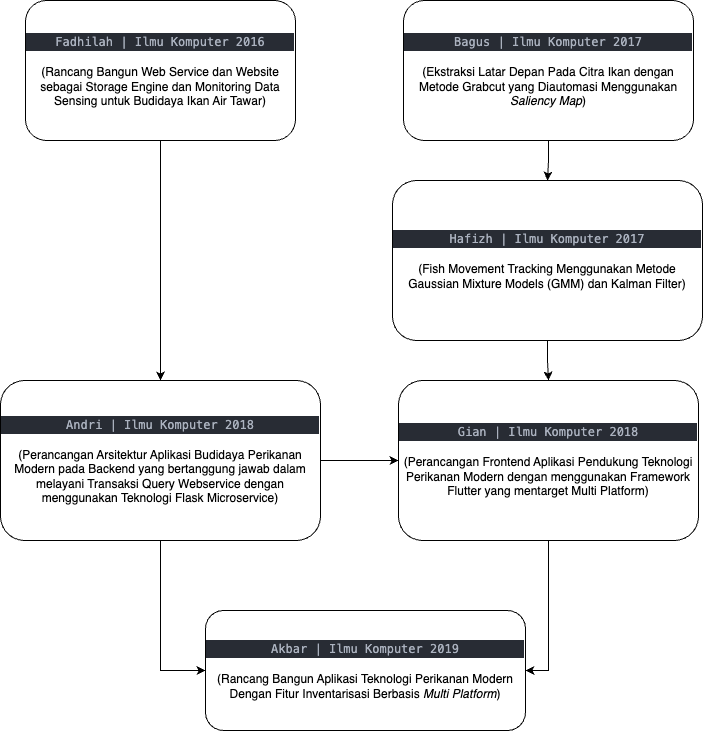
\includegraphics[width=0.7\textwidth]{gambar/akbar/research_tree.png}
	\caption{Diagram Alur Penelitian \textit{Aquaculture}}
\end{figure}

Pada diagram diatas, dapat dilihat urutan arah dari topik penelitian Aquaculture. Penelitian pertama kali dimulai oleh \citep{fadhil2021} dengan mengembangkan sebuah web service serta website yang berfungsi sebagai Storage Engine dan Monitoring Data Sensing untuk digunakan pada Budidaya Perikanan Air Tawar sebagai media penyimpanan data-data sensing dari sensor yang dikirimkan ke sistem serta memonitoringnya dalam bentuk table dan grafik real-time serta penelitian yang dilakukan oleh \citep{bagus2022} dengan tujuan untuk membangun sistem deteksi objek pada citra ikan dengan metode GrabCut yang telah diautomasi menggunakan \textit{saliency map}. 

Penelitian \citep{bagus2022} kemudian dilanjutkan oleh \citep{hafiz2021} yaitu merancang dan membangun sebuah sistem yang dapat melakukan pelacakan pergerakan ikan dengan menggunakan metode GMM dan Kalman Filter. Sementara penelitian \citep{fadhil2021} belum diterapkan pada aplikasi riset Aquaculture dalam waktu dekat sehingga penelitian yang dibuat oleh \citep{andri2022} dilakukan dengan membuat web service juga yang bertujuan untuk melayani transaksi query berupa monitoring budidaya perikanan yang dibarengi dengan penelitian \citep{gian2022} pada bagian perancangan \textit{frontend} sebagai pendukung pada aplikasi yang dikembangkan.

Dalam penelitian yang sudah berjalan ini, penulis mengembangkan penelitian yang dilakukan oleh \citep{andri2022} dan \citep{gian2022} dengan membuat fitur baru yaitu manajemen inventaris serta penentuan harga jual ikan dan penentuan upah petani ikan.

\section{Metode Penentuan Nilai Jual}

Dalam menentukan nilai jual, dapat digunakan rumus dibawah ini.





\section{Analisa Arsitektur Fitur}

Pada penelitian aplikasi yang sudah dikembangkan sebelumnya, terdapat use case yang menjelaskan konsep dari aplikasi yang ada pada gambar dibawah ini.

\begin{figure}[H]
	\centering
	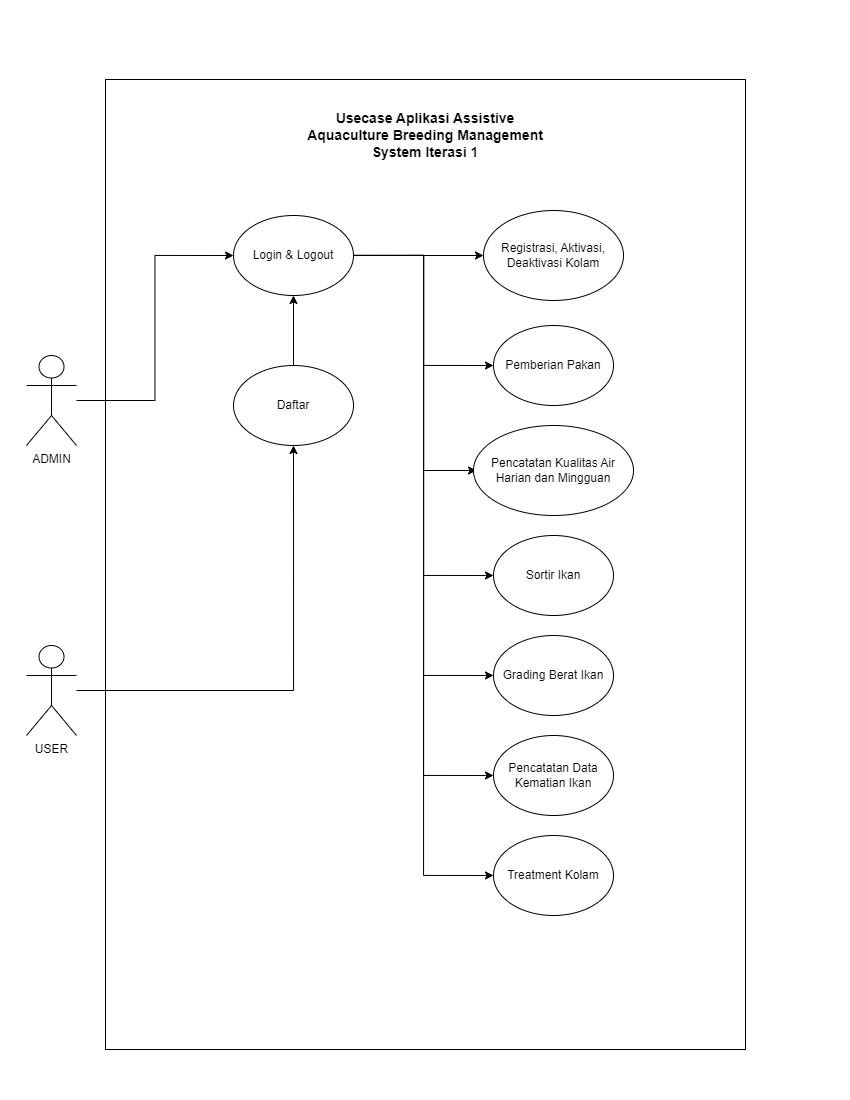
\includegraphics[width=0.7\textwidth]{gambar/akbar/usecase_iterasi_1.jpeg}
	\caption{Use Case Fitur Aplikasi pada Iterasi 1}
\end{figure}

Dari diagram use case tersebut, 

\section{Analisa Pengembangan Fitur}

Pada analisa arsitektur fitur yang ada di aplikasi sebelumnya, dapat dilengkapi dengan fitur inventaris yang akan dilakukan pada penelitian ini. Fitur tersebut memiliki use case diagram seperti berikut.

\begin{figure}[H]
	\centering
	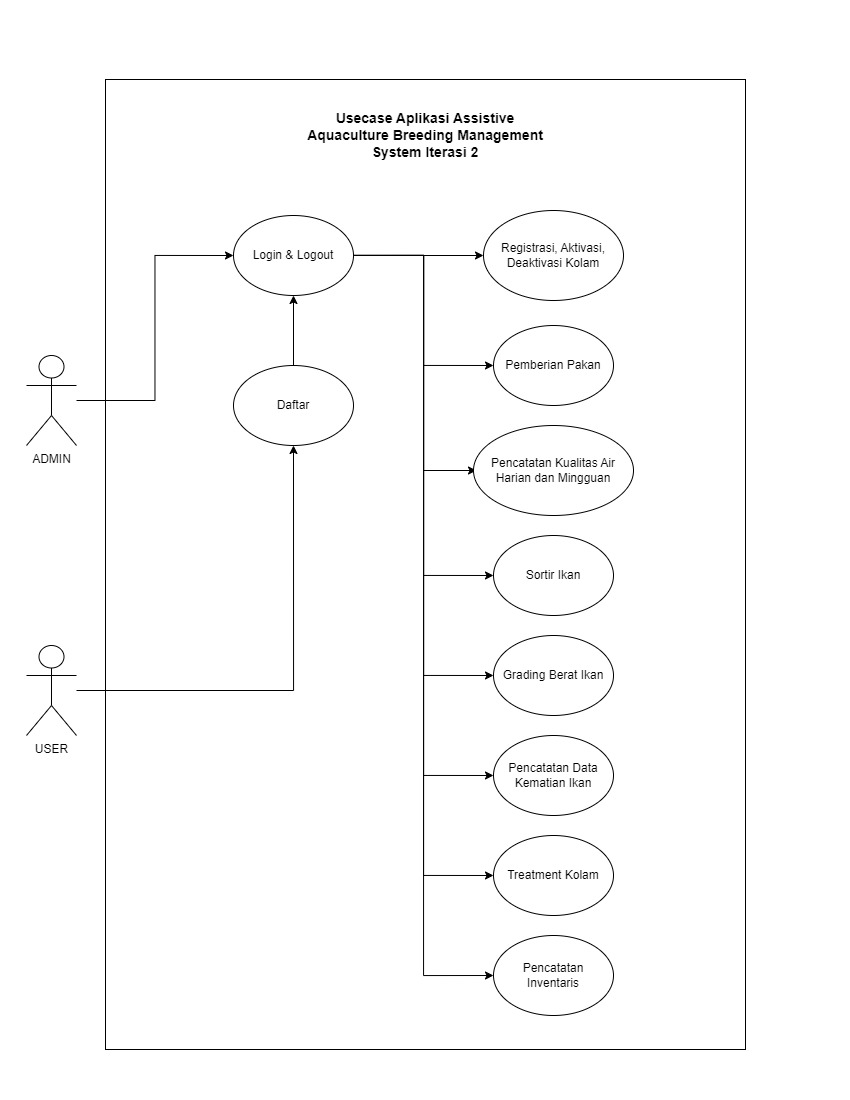
\includegraphics[width=0.7\textwidth]{gambar/akbar/usecase_iterasi_2.jpeg}
	\caption{Use Case Fitur Aplikasi pada Iterasi 2}
\end{figure}


% \section{Stories}

%     \subsection{Pencatatan Inventaris}

%     \begin{enumerate}
%         \item Bahan baku
%         \begin{enumerate}
%             \item Pakan
%             \item Bahan organik
%         \end{enumerate}
%         \item Listrik
%         \item Benih
%     \end{enumerate}

%     \subsection{Depresiasi Aset}

%     \begin{enumerate}
%         \item Kadaluarsa bahan baku
%         \item Penurunan kualitas
%     \end{enumerate}